\documentclass[../main/CT4S-EN-RU]{subfiles}

\begin{document}

\section{\caseENGRUS{Monoids}{ / }{Моноиды}}\label{sec:monoids}

\begin{blockENG}
A common way to interpret phenomena we see around us is to say that agents are acting on objects. For example, in a computer drawing program, the user {\em acts on} the canvas in certain prescribed ways. Choices of actions from an available list can be performed in sequence to transform one image into another. As another example, one might investigate the notion that time {\em acts on} the position of hands on a clock in a prescribed way. A first rule for actions is this: the performance of a sequence of several actions is itself the performance of an action—a more complex action, but an action nonetheless.
\end{blockENG}

\begin{blockRUS}
Общепринятым способом интерпретировать феномены, которые мы наблюдаем вокруг, является объяснение их воздействием некоторых факторов на объекты. Например, в программе компьютерной графики пользователь заранее определенными способами {\em воздействует на} область рисования. Выбор действий из списка всех доступных [в данной программе] может быть повторен многократно, преобразуя в результате одно изображение в другое. В качестве другого примера можно рассмотреть то, как время заранее определенным способом {\em воздействует на} положение стрелок на часах. Первое правило воздействия такое: проведение последовательно нескольких воздействий само является воздействием, — более сложным, но все равно воздействием.
\end{blockRUS}

\begin{blockENG}
Mathematical objects called {\em monoids} and {\em groups} are tasked with encoding the agent's perspective in all this, i.e. what the agent can do, and what happens when different actions are done in succession. A monoid can be constructed as a set of actions, together with a formula that encodes how a sequence of actions is itself considered an action. A group is the same as a monoid, except that every action is required to be reversible. In this section we concentrate on monoids; we will get to groups in Section~\ref{sec:groups}.
\end{blockENG}

\begin{blockRUS}
Математические объекты под названием {\em моноиды} и {\em группы} предназначены для формализации всего этого с точки зрения воздействующего фактора, т.е. вопроса, что наш фактор может проделать, и что происходит, когда различные действия выполнены последовательно. Моноид можно сконструировать из множества действий, взятого вместе с правилом, согласно которому последовательность действий может рассматриваться как одно действие. Кроме того, есть понятие группы — это то же, что и моноид, за исключением того, что мы дополнительно требуем, чтобы каждое действие в группе должно быть обратимым. В данном разделе мы сосредоточимся на моноидах; до групп мы доберемся в Разделе~\ref{sec:groups}.
\end{blockRUS}

%%%% Subsection %%%%

\subsection{\caseENGRUS{Definition and examples}{ / }{Определение и примеры}}

\begin{definitionENG}[Monoid]\label{def:monoid}\index{monoid}
A {\em monoid} is a sequence $(M,e,\star),$ where $M$ is a set, $e\in M$ is an element, and $\star\taking M\times M\to M$ is a function, such that the following conditions hold for all $m,n,p\in M$:
\begin{itemize}
\item $m\star e=m,$
\item $e\star m=m,$ and
\item $(m\star n)\star p=m\star(n\star p).$
\end{itemize}
We refer to $e$ as the {\em identity element}\index{monoid!identity element of} and to $\star$ as the {\em multiplication formula} for the monoid.\index{monoid!multiplication formula}%
\footnote{Although the function $\star\taking M\times M\to M$ is called the multiplication formula, it may have nothing to do with multiplication. It is nothing more than a formula for taking two inputs and returning an output; calling it “multiplication” is suggestive of its origins, rather than prescriptive of its behavior.}
We call the first two rules {\em identity laws} and the third rule the {\em associativity law} for monoids.
\end{definitionENG}

\begin{definitionRUS}[Моноид]\label{def:monoid}\index{моноид}
{\em Моноид} — это последовательность $(M,e,\star),$ где $M$ — множество, $e\in M$ — элемент, а $\star\taking M\times M\to M$ — функция такая, что следующие условия выполняются для всех $m,n,p\in M$:
\begin{itemize}
\item $m\star e=m,$
\item $e\star m=m,$
\item $(m\star n)\star p=m\star(n\star p).$
\end{itemize}
Мы называем элемент $e$ — {\em единицей}\index{моноид!единица}, а $\star$ — {\em правилом умножения} данного моноида.\index{моноид!правило умножения}%
\footnote{Хотя функция $\star\taking M\times M\to M$ называется правилом умножения, она может не иметь ничего общего с умножением. Это не более, чем алгоритм, берущий два исходных значения и возвращающий результат; именование его «умножением» должно быть скорее намеком на его истоки, а не требованием к его поведению.}
Мы называем первые два условия {\em свойствами единицы}, а третье {\em ассоциативным законом} для моноидов.%
\endnote{
Немного математического жаргона: если зафиксирован определенный моноид $(M,e,\star),$ то говорят, что на множестве $M$ задана структура моноида, а само множество $M$ называется носителем этой структуры.
}
\end{definitionRUS}

\begin{remarkENG}
To be pedantic, the conditions from Definition~\ref{def:monoid} should be stated
\begin{itemize}
\item $\star(m,e)=m,$
\item $\star(e,m)=m,$ and
\item $\star(\star(m,n),p)=\star(m,(\star(n,p)).$
\end{itemize}
The way they are written in Definition~\ref{def:monoid} is called {\em infix notation},\index{infix notation} and we often use infix notation without mentioning it. That is, given a function $\cdot\taking A\times B\to C,$ we may write $a\cdot b$ rather than $\cdot(a,b).$
\end{remarkENG}

\begin{remarkRUS}
Если подходить к вопросу более формально, условия из Определения~\ref{def:monoid} следовало бы записать так:
\begin{itemize}
\item $\star(m,e)=m,$
\item $\star(e,m)=m,$
\item $\star(\star(m,n),p)=\star(m,(\star(n,p)).$
\end{itemize}
В Определении~\ref{def:monoid}, однако, использован способ обозначения под названием {\em инфиксная нотация}\index{инфиксная нотация}, и он часто будет появляться без дополнительных предупреждений. В частности, для заданной функции $\cdot\taking A\times B\to C$ мы пишем $a\cdot b$ вместо $\cdot(a,b).$
\end{remarkRUS}

\begin{exampleENG}[Additive monoid of natural numbers]\label{ex:monoid 0}\index{monoid!additive natural numbers}
Let $M=\NN$ be the set of natural numbers. Let $e=0$ and let $\star\taking M\times M\to M$ denote addition, so that $\star(4,18)=22.$ Then the equations $m\star 0=m$ and $0\star m=m$ hold, and $(m\star n)\star p=m\star (n\star p).$ By assigning $e$ and $\star$ in this way, we have “given $\NN$ the structure of a monoid”.
\end{exampleENG}

\begin{exampleRUS}[Аддитивный моноид натуральных чисел]\label{ex:monoid 0}\index{моноид!натуральных чисел!аддитивный}
Пусть $M=\NN$ — это множество натуральных чисел. Положим $e=0,$ а $\star\taking M\times M\to M$ пусть обозначает сложение, например, $\star(4,18)=22.$ Тогда равенства $m\star 0=m$ и $0\star m=m$ действительно выполняются, также как и $(m\star n)\star p=m\star (n\star p).$ Выбрав $e$ и $\star$ подобным образом, мы «придаем $\NN$ структуру моноида».
\end{exampleRUS}

\begin{remarkENG}
Sometimes we are working with a monoid $(M,e,\star),$ and the identity $e$ and multiplication $\star$ are somehow clear from context. In this case we might refer to the set $M$ as though it were the whole monoid. For example, if we were discussing the monoid from Example~\ref{ex:monoid 0}, we might refer to it as $\NN.$ The danger comes because sets may have multiple monoid structures, as we see below in Exercise~\ref{exc:monoid 1}.
\end{remarkENG}

\begin{remarkRUS}
Иногда мы работаем с фиксированным моноидом $(M,e,\star),$ при этом единица $e$ и умножение $\star$ некоторым образом ясны из контекста. В подобных случаях мы будем обозначать моноид тем же именем, что и множество $M,$ как если бы само множество было моноидом. Например, при обсуждении моноида из Примера~\ref{ex:monoid 0}, мы могли бы сослаться на него, как на $\NN.$ Здесь, однако, присутствует известная опасность, поскольку одно множество может иметь много разных структур моноида, в чем мы убедимся ниже, в Примере~\ref{exc:monoid 1}.
\end{remarkRUS}

\begin{exampleENG}[Non-monoid]
If $M$ is a set, we might call a function $f\taking M\times M\to M$ an {\em operation on $M$}. For example, if $M=\NN$ is the set of natural numbers, we can consider the operation $f\taking\NN\to\NN$ called exponentiation. For example $f(2,5)=2*2*2*2*2=32$ and $f(7,2)=49.$ This is indeed an operation, but it is not part of any monoid. For one thing there is no possible unit. Trying the obvious choice of $e=1,$ we see that $a^1=a$ (good), but that $1^a=1$ (bad: we need it to be $a$). For another thing, this operation is not associative because in general $a^{b^c}\neq (a^b)^c.$ For example, $2^{1^2}=2$ but $(2^1)^2=4.$

One might also attempt to consider an operation $f\taking M\times M\to M$ that, upon closer inspection, aren't even operations. For example, if $M=\ZZ$ then exponentiation is not even an operation. Indeed, $f(2,-1)=2^{-1}=\frac{1}{2},$ and this is not an integer. To have a function $f\taking M\times M\to M,$ we need that every element of the domain, in this case every pair of integers, has an output under $f.$ So there is no such function $f.$
\end{exampleENG}

\begin{exampleRUS}[Не моноид]
Если $M$ — это множество, мы называем функцию $f\taking M\times M\to M$ {\em операцией на $M$}. В частности, если $M=\NN$ — множество натуральных чисел, мы можем рассмотреть операцию возведения в степень $f\taking\NN\to\NN.$ Например, $f(2,5)=2*2*2*2*2=32$ и $f(7,2)=49.$ Это в самом деле операция, но она не является частью никакого моноида. Во-первых, у нее нет единицы. Попробовав очевидный вариант $e=1,$ мы видим, что $a^1=a$ (хорошо), но, с другой стороны, $1^a=1$ (плохо: нужно, чтобы получилось $a$). Во-вторых, эта операция не ассоциативна, поскольку в общем случае $a^{b^c}\neq (a^b)^c.$ Например, $2^{1^2}=2,$ но $(2^1)^2=4.$

Кроме того, можно даже рассмотреть такую операцию $f\taking M\times M\to M,$ которая, при ближайшем рассмотрении, не является операцией. Например, если $M=\ZZ,$ то возведение в степень не является операцией. Действительно, $f(2,-1)=2^{-1}=\frac{1}{2},$ и это не целое число. Чтобы у нас была на самом деле функция $f\taking M\times M\to M,$ нужно, чтобы для каждого элемента области определения, в данном случае — для любой пары целых чисел, у нас получался результат из $M.$ Но такой функции $f,$ действующей на целых числах, нет.
\end{exampleRUS}

\begin{exerciseENG}\label{exc:monoid 1}
Let $M=\NN$ be the set of natural numbers. Taking $e=1,$ come up with a formula for $\star$ that gives $\NN$ the structure of a monoid.
\end{exerciseENG}

\begin{exerciseRUS}\label{exc:monoid 1}
Пусть $M=\NN$ — множество натуральных чисел. Выбрав $e=1,$ предложите формулу для $\star,$ которая задает на $\NN$ структуру моноида.
\end{exerciseRUS}

\begin{exerciseENG}
Come up with an operation on the set $M=\{1,2,3,4\},$ i.e. a legitimate function $f\taking M\times M\to M,$ such that $f$ cannot be the multiplication formula for a monoid on $M.$ That is, either it is not associative, or no element of $M$ can serve as a unit.
\end{exerciseENG}

\begin{exerciseRUS}
Предложите операцию на множестве $M=\{1,2,3,4\},$ другими словами — корректную функцию $f\taking M\times M\to M$ такую, что $f$ не может быть умножением для моноида на $M.$ То есть такую, которая либо не была бы ассоциативной, либо ни один элемент в $M$ не был бы ее единицей.
\end{exerciseRUS}

\begin{exerciseENG}\label{ex:commutative monoid}
In both Example~\ref{ex:monoid 0} and Exercise~\ref{exc:monoid 1}, the monoids $(M,e,\star)$ satisfied an additional rule called {\em commutativity},\index{monoid!commutative} namely $m\star n=n\star m$ for every $m,n\in M.$ There is a monoid $(M,e,\star)$ lurking in linear algebra textbooks that is not commutative; if you have background in linear algebra try to answer this: what $M, e,$ and $\star$ might I be referring to?
\end{exerciseENG}

\begin{exerciseRUS}\label{ex:commutative monoid}
В Упражнении~\ref{ex:monoid 0} и Упражнении~\ref{exc:monoid 1} для упомянутых там моноидов $(M,e,\star)$ выполняется дополнительное свойство, называемое {\em коммутативностью}\index{моноид!коммутативный}, а именно $m\star n=n\star m$ для любых $m,n\in M.$ В учебниках по линейной алгебре обсуждается моноид $(M,e,\star),$ не являющийся коммутативным; если вы знакомы с линейной алгеброй, попытайтесь ответить на вопрос: каковы подходящие для этого $M, e,$ и $\star$?
\end{exerciseRUS}

\begin{exerciseENG}
Recall the notion of commutativity for monoids from Exercise~\ref{ex:commutative monoid}.
\sexc What is the smallest set $M$ that you can give the structure of a non-commutative monoid?
\item What is the smallest set $M$ that you can give the structure of a monoid?
\endsexc
\end{exerciseENG}

\begin{exerciseRUS}
Вспомним понятие коммутативности моноидов из Упражнения~\ref{ex:commutative monoid}.
\sexc Каково наименьшее множество $M,$ которому можно придать структуру некоммутативного моноида?
\item Каково наименьшее множество $M,$ которому можно придать структуру моноида?
\endsexc
\end{exerciseRUS}

\begin{exampleENG}[Trivial monoid]\label{ex:trivial monoid}
There is a monoid with only one element, $M=(\{e\},e,\star)$ where $\star\taking\{e\}\times\{e\}\to\{e\}$ is the unique function. We call this monoid {\em the trivial monoid},\index{monoid!trivial} and sometimes denote it $\ul{1}.$
\end{exampleENG}

\begin{exampleRUS}[Тривиальный моноид]\label{ex:trivial monoid}
Имеется моноид с одним элементом, $M=(\{e\},e,\star),$ где $\star\taking\{e\}\times\{e\}\to\{e\}$ — единственная функция. Мы называем этот моноид {\em тривиальным моноидом},\index{моноид!тривиальный} и иногда обозначаем его $\ul{1}.$
\end{exampleRUS}

\begin{exampleENG}
Suppose that $(M,e,\star)$ is a monoid. Given elements $m_1,m_2,m_3,m_4$ there are five different ways to parenthesize the product $m_1\star m_2\star m_3\star m_4,$ and the associativity law for monoids will show them all to be the same. We have
\begin{align*}
((m_1\star m_2)\star m_3)\star m_4&=(m_1\star m_2)\star (m_3\star m_4)\\
&=(m_1\star(m_2\star m_3))\star m_4\\
&=m_1\star(m_2\star (m_3\star m_4))\\
&=m_1\star((m_2\star m_3)\star m_4)
\end{align*}

In fact, the product of any list of monoid elements is the same, regardless of parenthesization. Therefore, we can unambiguously write $m_1m_2m_3m_4m_5$ rather than any given parenthesization of it. This is known as the \href{http://en.wikipedia.org/wiki/Coherence_theorem}{\text coherence theorem} and can be found in \cite{Mac}.
\end{exampleENG}

\begin{exampleRUS}
Предположим, что $(M,e,\star)$ — это моноид. Для заданных элементов $m_1,m_2,m_3,m_4$ имеется пять различных способов расстановки скобок в произведении $m_1\star m_2\star m_3\star m_4,$ при этом закон ассоциативности для моноидов гарантирует, что все они равны. Выполняются равенства:
\begin{align*}
((m_1\star m_2)\star m_3)\star m_4&=(m_1\star m_2)\star (m_3\star m_4)\\
&=(m_1\star(m_2\star m_3))\star m_4\\
&=m_1\star(m_2\star (m_3\star m_4))\\
&=m_1\star((m_2\star m_3)\star m_4)
\end{align*}

Более общо, произведения любого списка элементов моноида совпадают, независимо от расстановки скобок. Таким образом, мы можем непротиворечиво писать $m_1m_2m_3m_4m_5$ совсем без скобок. Этот факт известен под названием \href{http://en.wikipedia.org/wiki/Coherence_theorem}{\text теоремы когеррентности} и может быть найден в \cite{Mac}.
\end{exampleRUS}

%% Subsubsection %%

\subsubsection{\caseENGRUS{Free monoids and finitely presented monoids}{ / }{Свободные и конечно представимые моноиды}}\label{sec:free monoid}

\begin{definitionENG}\label{def:list}\index{list}
Let $X$ be a set. A {\em list in $X$} is a pair $(n,f)$ where $n\in\NN$ is a natural number (called the {\em length of the list}) and $f\taking\ul{n}\to X$ is a function, where $\ul{n}=\{1,2,\ldots,n\}.$ We may denote such a list by
$$(n,f)=[f(1),f(2),\ldots,f(n)].$$
The {\em empty list} is the unique list in which $n=0$; we may denote it by $[\,].$ Given an element $x\in X$ the {\em singleton list on $x$} is the list $[x].$ Given a list $L=(n,f)$ and a number $i\in\NN$ with $i\leq n,$ the {\em $i$th entry of $L$} is the element $f(i)\in X.$ \index{entry!in list}

Given two lists $L=(n,f)$ and $L'=(n',f'),$ define the {\em concatenation of $L$ and $L'$}\index{list!concatenation}\index{concatenation!of lists}, denoted $L\plpl L',$\index{a symbol!$\plpl$} to be the list $(n+n',f\plpl f'),$ where $f\plpl f'\taking \ul{n+n'}\to X$ is given on $i\leq n+n'$ by
$$(f\plpl f')(i):=
\begin{cases}
f(i)&\tn{ if }i\leq n\\
f'(i-n)&\tn{ if }i\geq n+1
\end{cases}
$$
\end{definitionENG}

\begin{definitionRUS}\label{def:list}\index{list}
Пусть $X$ — это множество. {\em Список с элементами из $X$} — это пара $(n,f),$ где $n\in\NN$ — натуральное число (называемое {\em длиной списка}), а $f\taking\ul{n}\to X$ — функция, где $\ul{n}=\{1,2,\ldots,n\}.$ Его можно обозначить так:
$$(n,f)=[f(1),f(2),\ldots,f(n)].$$
{\em Пустой список} — это единственный список длины $n=0$; его можно обозначить $[\,].$ Для заданного элемента $x\in X$ {\em одноэлементный список $x$} — это список $[x]$ длины $n=1$. Если задан список $L=(n,f)$ и число $i\in\NN,$ причем $i\leq n,$ то {\em $i$-м элементом $L$} называется значение $f(i)\in X.$ \index{элемент!списка}

Множество всех списков с элементами из $X$ обозначается $\List(X).$

Для заданных двух списков $L=(n,f)$ и $L'=(n',f'),$ определим {\em конкатенацию $L$ и $L'$}\index{список!конкатенация}\index{конкатенация!списков}, обозначаемую $L\plpl L',$\index{символ!$\plpl$} как список $(n+n',f\plpl f'),$ где $f\plpl f'\taking \ul{n+n'}\to X$ задано на $i\leq n+n'$ как
$$(f\plpl f')(i):=
\begin{cases}
f(i),&\tn{если}i\leq n\\
f'(i-n),&\tn{если}i\geq n+1
\end{cases}
$$
\end{definitionRUS}

\begin{exampleENG}
Let $X=\{a,b,c,\ldots,z\}.$ The following are elements of $\List(X)$: $$[a,b,c],\;\; [p],\;\; [p,a,a,a,p],\;\; [\,],\;\;\dots$$ The concatenation of $[a,b,c]$ and $[p,a,a,a,p]$ is $[a,b,c,p,a,a,a,p].$ The concatenation of any list $A$ with $[\,]$ is just $A.$
\end{exampleENG}

\begin{exampleRUS}
Пусть $X=\{a,b,c,\ldots,z\}.$ Вот примеры элементов $\List(X)$: $$[a,b,c],\;\; [p],\;\; [p,a,a,a,p],\;\; [\,],\;\;\dots$$ Конкатенацией списков $[a,b,c]$ и $[p,a,a,a,p]$ будет $[a,b,c,p,a,a,a,p].$ Конкатенацией любого списка $A$ с пустым списком $[\,]$ будет само $A.$
\end{exampleRUS}

\begin{definitionENG}\label{def:free monoid}\index{monoid!free}
Let $X$ be a set. The {\em free monoid generated by $X$} is the sequence $M:=(\List(X),[\,],\plpl),$ where $\List(X)$ is the set of lists of elements in $X,$ where $[\,]\in\List(X)$ is the empty list, and where $\plpl$ is the operation of list concatenation. We refer to $X$ as the set of generators for the monoid $M.$
\end{definitionENG}

\begin{definitionRUS}\label{def:free monoid}\index{monoid!free}
Пусть $X$ — это множество. {\em Свободный моноид, порожденный $X$} — это последовательность $M:=(\List(X),[\,],\plpl),$ где носитель $\List(X)$ — множество списков с элементами из $X,$ единица $[\,]\in\List(X)$ — пустой список, а $\plpl$ — операция конкатенации. Мы будем говорить об $X$ как о множестве, порождающем моноид $M,$ а о его элементах — как о порождающих.
\end{definitionRUS}

\begin{exerciseENG}
Let $\singleton$ denote a one-element set.
\sexc What is the free monoid generated by $\singleton?$
\item What is the free monoid generated by $\emptyset?$
\endsexc
\end{exerciseENG}

\begin{exerciseRUS}
Пусть $\singleton$ обозначает множество с единственным элементом.
\sexc Каким будет свободный моноид, порожденный $\singleton?$
\item Каким будет свободный моноид, порожденный $\emptyset?$
\endsexc
\end{exerciseRUS}

\begin{blockENG}
In the definition below, we will define a monoid $M$ by specifying some generators and some relations. Lists of generators provide us all the possible ways to write elements of $M.$ The relations allow us to have two such ways of writing the same element. The following definition is a bit dense, so see Example~\ref{ex:presented monoid} for a concrete example.
\end{blockENG}

\begin{blockRUS}
Ниже мы определяем моноид $M,$ задав определенные порождающие и некоторые отношения между ними. Разные списки порождающих дают нам все возможные способы записать элементы $M$ [в виде произведения других элементов]. Отношения позволяют иметь несколько способов записи для одного элемента.%
\endnote{
TODO: написать про конгруэнции
}
Следующее определение достаточно абстрактно и тяжеловесно, для конкретных примеров см. Пример~\ref{ex:presented monoid}.
\end{blockRUS}

\begin{definitionENG}[Presented monoid]\label{def:presented monoid}\index{monoid!presented}
Let $G$ be a finite set, let $n\in\NN$ be a natural number,%
\footnote{The number $n\in\NN$ is going to stand for the number of relations we declare.}
and for each $1\leq i\leq n,$ let $m_i$ and $m_i'$ be elements of $\List(G).$%
\footnote{Each $m_i$ and $m_i'$ are going to be made equal in the set $M.$}
The {\em monoid presented by generators $G$ and relations $\{(m_i,m_i')\|1\leq i\leq n\}$} is the monoid $\mcM=(M,e,\star)$ defined as follows. Let $\sim$ denote the equivalence relation on $\List(G)$ generated by $\{(xm_iy\sim xm_i'y)\|x,y\in\List(G), 1\leq i\leq n\},$ and define $M=\List(G)/\sim.$ Let $e=[\,]$ and let $a * b$ be obtained by concatenating representing lists.
\end{definitionENG}

\begin{definitionRUS}[Задание моноида]\label{def:presented monoid}\index{monoid!presented}
Пусть $G$ — это конечное множество, а $n\in\NN$ — натуральное число,%
\footnote{Число $n\in\NN$ должно обозначать количество вводимых отношений.}
и для каждого $1\leq i\leq n$ пусть $m_i$ и $m_i'$ будут элементами $\List(G).$%
\footnote{Каждый $m_i$ и $m_i'$ будут объявлены совпадающими в $M.$}
{\em Моноид, заданный порождающими $G$ и отношениями $\{(m_i,m_i')\|1\leq i\leq n\}$} — это моноид $\mcM=(M,e,\star),$ определяемый следующим образом. Пусть $\sim$ обозначает отношение эквивалентности на $\List(G),$ порожденное $\{(xm_iy\sim xm_i'y)\|x,y\in\List(G), 1\leq i\leq n\};$ определим тогда $M=\List(G)/\sim.$ Определим также $e=[\,],$ а умножение $a * b$ получается из конкатенации представляющих списков. 
\end{definitionRUS}

\begin{remarkENG}
Every free monoid is a presented monoid, because we can just take the set of relations to be empty.
\end{remarkENG}

\begin{remarkRUS}
Каждый свободный моноид обладает заданием, поскольку множество отношений можно взять пустым.
\end{remarkRUS}

\begin{exampleENG}\label{ex:presented monoid}
Let $G=\{a,b,c,d\}.$ Think of these as buttons that can be pressed. The free monoid $\List(G)$ is the set of all ways of pressing buttons, e.g. pressing $a$ then $a$ then $c$ then $c$ then $d$ corresponds to the list $[a,a,c,c,d].$ The idea of presented monoids is that you notice that pressing $[a,a,c]$ always gives the same result as pressing $[d,d].$ You also notice that pressing $[c,a,c,a]$ is the same thing as doing nothing.

In this case, we would have $m_1=[a,a,c],$ $m_1'=[d,d],$ and $m_2=[c,a,c,a], m_2'=[\,]$ and relations $\{(m_1,m_1'), (m_2,m_2')\}.$ Really this means that we're equating $m_1$ with $m_1'$ and $m_2$ with $m_2',$ which for convenience we'll write out:
$${\color{blue}{[a,a,c]}}={\color{blue}{[d,d]}}\hsp\tn{and}\hsp{\color{red}{[a,c,a,c]}}={\color{red}{[\,]}}
$$

To see how this plays out, we give an example of a calculation in $M=\List(G)/\sim.$ Namely,
\begin{align*}
[b,c,b,{\color{blue}{d,d}},a,c,a,a,c,d] = [b,c,b,a,a,{\color{red}{c,a,c,a}},a,c,d] &= [b,c,b,a,{\color{blue}{a,a,c}},d]\\
&= [b,c,b,a,d,d,d].
\end{align*}
\end{exampleENG}

\begin{exampleRUS}\label{ex:presented monoid}
Пусть $G=\{a,b,c,d\}.$ Будем думать о них, как о нажимаемых кнопках. Свободный моноид $\List(G)$ — это множество всех способов нажимать кнопки, например, нажатие $a,$ затем $a,$ затем $c,$ затем $c,$ затем $d$ соответствует списку $[a,a,c,c,d].$ Идея задания моноида в том, что мы можем заметить, что нажатие $[a,a,c]$ всегда дает тот же самый результат, что и нажатие $[d,d].$ Мы можем также узнать о том, что нажатие $[c,a,c,a]$ равносильно отсутствию нажатий.

В таком случае нам следовало бы взять $m_1=[a,a,c],$ $m_1'=[d,d],$ и $m_2=[c,a,c,a],$ $m_2'=[\,]$ с отношениями $\{(m_1,m_1'), (m_2,m_2')\}.$ На самом деле это означает, что мы приравниваем $m_1$ с $m_1'$ и $m_2$ с $m_2',$ что для удобства можно записать так:
$${\color{blue}{[a,a,c]}}={\color{blue}{[d,d]}}\hsp\tn{и}\hsp{\color{red}{[a,c,a,c]}}={\color{red}{[\,]}}
$$

Чтобы увидеть, как это работает, возьмем для примера такое вычисление в $M=\List(G)/\sim$
\begin{align*}
[b,c,b,{\color{blue}{d,d}},a,c,a,a,c,d] = [b,c,b,a,a,{\color{red}{c,a,c,a}},a,c,d] &= [b,c,b,a,{\color{blue}{a,a,c}},d]\\
&= [b,c,b,a,d,d,d].
\end{align*}
\end{exampleRUS}

\begin{applicationENG}[Buffer]\label{app:buffer}
Let $G=\{a,b,c,\ldots\,z\}.$ Suppose we have a \href{http://en.wikipedia.org/wiki/Data_buffer}{\text buffer} of 32 characters and we want to consider the set of lists of length at most 32 to be a monoid. We simply have to decide what happens when someone types a list of length more than 32.

One option is to say that the last character typed overwrites the 32nd entry, $$[a_1,a_2,\ldots,a_{31},a_{32},b]\sim_1[a_1,a_2,\ldots,a_{31},b].$$ Another option is to say that any character typed after\_32 entries is discarded, $$[a_1,a_2,\ldots,a_{31},a_{32},b]\sim_2[a_1,a_2,\ldots,a_{31},a_{32}].$$ Both of these yield finitely presented monoids, generated by $G.$ (In case it's useful, the number of necessary relations in both cases is $26^{33}.$)
\end{applicationENG}

\begin{applicationRUS}[Буфер]\label{app:buffer}
Пусть $G=\{a,b,c,\ldots\,z\}.$ Предположим, у нас есть \href{https://ru.wikipedia.org/wiki/%D0%91%D1%83%D1%84%D0%B5%D1%80_(%D0%B8%D0%BD%D1%84%D0%BE%D1%80%D0%BC%D0%B0%D1%82%D0%B8%D0%BA%D0%B0)}{\text буфер} из $32$ символов, и мы хотим рассматривать в качестве моноида множество списков длиной не более $32.$ Нам только потребуется решить, что будет происходить, когда некто вводит список длиной более $32$.

Один из вариантов — сказать, что последний записанный символ должен перезаписывать последний, $32$-й элемент, $$[a_1,a_2,\ldots,a_{31},a_{32},b]\sim_1[a_1,a_2,\ldots,a_{31},b].$$ Другой вариант — сказать, что все символы после первых 32-х должны быть отброшены, $$[a_1,a_2,\ldots,a_{31},a_{32},b]\sim_2[a_1,a_2,\ldots,a_{31},a_{32}].$$ Оба способа порождают конечно заданные моноиды, порожденные $G.$ (Число необходимых отношений в обоих случаях равняется $26^{33}.$)
\end{applicationRUS}

\begin{exerciseENG}\label{exc:buffer3}
Let's consider the buffer concept again (see Application~\ref{app:buffer}), but this time only having size 3 rather than size 32. Show using Definition~\ref{def:presented monoid} that with relations given by $\sim_1$ we indeed have $[a,b,c,d,e,f]=[a,b,f]$ and that with relations given by $\sim_2$ we indeed have $[a,b,c,d,e,f]=[a,b,c].$
\end{exerciseENG}

\begin{exerciseRUS}\label{exc:buffer3}
Еще раз рассмотрим понятие буфера (см. Применение~\ref{app:buffer}), но на этот раз с тремя элементами вместо $32$-х. Покажите, используя Определение~\ref{def:presented monoid}, что с отношениями $\sim_1$ мы получим $[a,b,c,d,e,f]=[a,b,f],$ а с отношениями $\sim_2$ будет выполняться $[a,b,c,d,e,f]=[a,b,c].$
\end{exerciseRUS}

\begin{exerciseENG}
Let $K:=\{BS,a,b,c,\ldots,z\},$ a set having 27 elements. Suppose you want to think of $BS\in K$ as the “backspace key” and the elements $a,b,\ldots z\in K$ as the letter keys on a keyboard. Then the free monoid $\List(K)$ is not quite appropriate as a model because we want $[a,b,d,BS]=[a,b].$
\sexc Choose a set of relations for which the monoid presented by generators $K$ and the chosen relations is appropriate to this application.
\item Under your relations, how does $[BS]$ compare with $[\,]?$ Is that suitable?
\endsexc
\end{exerciseENG}

\begin{exerciseRUS}
Пусть $K:=\{BS,a,b,c,\ldots,z\}$ — это множество, имеющее $27$ элементов. Предположим, мы хотим думать о $BS\in K$ как о клавише «backspace» (забой), а об элементах $a,b,\ldots z\in K$ — как об алфавитных клавишах на клавиатуре. Тогда свободный моноид $\List(K)$ не является подходящей моделью, поскольку мы хотим, чтобы $[a,b,d,BS]=[a,b].$
\sexc Выберите множество отношений так, чтобы моноид, заданный порождающими $K$ и этими отношениями, подходил к нашему прикладному примеру.
\item С этими отношениями, будет ли $[BS]$ равен $[\,]?$ Подходит ли это нам?
\endsexc
\end{exerciseRUS}

%% Subsubsection %%

\subsubsection{\caseENGRUS{Cyclic monoids}{ / }{Циклические моноиды}}

\begin{definitionENG}
A monoid is called {\em cyclic}\index{monoid!cyclic} if it has a presentation involving only one generator.
\end{definitionENG}

\begin{definitionRUS}
Моноид называется {\em циклическим}\index{моноид!циклический}, если он порожден одним элементом, т.е. имеет задание с одноэлементным множеством порождающих.
\end{definitionRUS}

\begin{exampleENG}\label{ex:cyclic}
Let $Q$ be a symbol; we look at some cyclic monoids generated by $\{Q\}.$ With no relations the monoid would be the free monoid on one generator, and would have underlying set $\{[\,],[Q],[Q,Q],[Q,Q,Q],\ldots\},$ with identity element $[\,]$ and multiplication given by concatenation (e.g. $[Q,Q,Q]\plpl[Q,Q]=[Q,Q,Q,Q,Q]$). This is just $\NN,$ the additive monoid of natural numbers.

With the really strong relation $[Q]\sim[\,]$ we would get the trivial monoid, a monoid having only one element (see Example~\ref{ex:trivial monoid}).

Another possibility is given in the first part of Example~\ref{ex:clocks}, where the relation $Q^{12}\sim[\,]$ is used, where $Q^{12}$ is shorthand for $[Q,Q,Q,Q,Q,Q,Q,Q,Q,Q,Q,Q].$
\end{exampleENG}

\begin{exampleRUS}\label{ex:cyclic}
Пусть $Q$ — это символ; взглянем на некоторые циклические моноиды, порожденные $\{Q\}.$ Без отношений мы получим просто свободный моноид с одним порождающим, имеющий множество-носитель $\{[\,],[Q],[Q,Q],[Q,Q,Q],\ldots\},$ единицу $[\,]$ и умножение, заданное конкатенацией (например, $[Q,Q,Q]\plpl[Q,Q]=[Q,Q,Q,Q,Q]$). Попросту говоря, это $\NN,$ аддитивный моноид натуральных чисел.

С самым сильным отношением $[Q]\sim[\,]$ мы получим тривиальный моноид, т.е. моноид, имеющий только один элемент (см. Пример~\ref{ex:trivial monoid}).

Еще одна возможность дается первой частью Примера~\ref{ex:clocks}, где использовано отношение $Q^{12}\sim[\,],$ где $Q^{12}$ — сокращение для $[Q,Q,Q,Q,Q,Q,Q,Q,Q,Q,Q,Q].$
\end{exampleRUS}

\begin{exampleENG}\label{ex:cyclic monoid (7,4)}
Consider the cyclic monoid with generator $Q$ and relation $Q^7=Q^4.$ This monoid has seven elements, $\{e=Q^0,Q=Q^1, Q^2, Q^3, Q^4, Q^5, Q^6\},$ and we know that $Q^6\star Q^5=Q^7*Q^4=Q^4*Q^4=Q^7*Q=Q^5.$ One might depict this monoid as follows
$$\xymatrix@=15pt{
\LMO{e}\ar[rr]&&\LMO{Q}\ar[rr]&&\LMO{Q^2}\ar[rr]&&\LMO{Q^3}\ar[rr]&&\LMO{Q^4}\ar[dr]\\
&&&&&&&\LMO{Q^6}\ar[ur]&&\LMO{Q^5}\ar[ll]
}
$$
To see the mathematical source of this intuitive depiction, see Example~\ref{ex:yoneda for cyclic monoid}.
\end{exampleENG}

\begin{exampleRUS}\label{ex:cyclic monoid (7,4)}
Рассмотрим циклический моноид с порождающим $Q$ и отношением $Q^7=Q^4.$ Этот моноид имеет семь элементов, $\{e=Q^0,Q=Q^1, Q^2, Q^3, Q^4, Q^5, Q^6\},$и мы знаем, что $Q^6\star Q^5=Q^7*Q^4=Q^4*Q^4=Q^7*Q=Q^5.$ Изобразить этот моноид можно так:
$$\xymatrix@=15pt{
\LMO{e}\ar[rr]&&\LMO{Q}\ar[rr]&&\LMO{Q^2}\ar[rr]&&\LMO{Q^3}\ar[rr]&&\LMO{Q^4}\ar[dr]\\
&&&&&&&\LMO{Q^6}\ar[ur]&&\LMO{Q^5}\ar[ll]
}
$$
Чтобы разобраться с математическим источником этой интуитивной картинки, см. Пример~\ref{ex:yoneda for cyclic monoid}.
\end{exampleRUS}

\begin{exerciseENG}[Classify the cyclic monoids]\label{exc:classify cyclic}
Classify all the cyclic monoids up to isomorphism. That is, come up with a naming system such that every cyclic monoid can be given a name in your system, such that no two non-isomorphic cyclic monoids have the same name, and such that no name exists in the system unless it refers to a cyclic monoid.

Hint: one might see a pattern in which the three monoids in Example~\ref{ex:cyclic} correspond respectively to $\infty,$ $1,$ and $12,$ and then think “Cyclic monoids can be classified by (i.e. systematically named by elements of) the set $\NN\sqcup\{\infty\}.$” That idea is on the right track, but is not correct.
\end{exerciseENG}

\begin{exerciseRUS}[Классификация циклических моноидов]\label{exc:classify cyclic}
Классифицируйте все циклические моноиды с точностью до изоморфизма. Другими словами, предложите систему названий такую, чтобы каждый циклический моноид получил имя в вашей системе, при этом неизоморфиные моноиды не должны получить одно имя, и не должно быть ни одного имени, не означающего циклический моноид.

Подсказка: можно заметить общую закономерность, согласно которой три моноида в Примере~\ref{ex:cyclic} можно обозначить соответственно $\infty,$ $1,$ и $12,$ и затем подумать «Циклические моноиды могут быть классифицированы (т.е. систематически названы элементами) множества $\NN\sqcup\{\infty\}.$» Эта идея ведет в правильном направлении, хотя буквально она не верна.
\end{exerciseRUS}

%%%% Subsection %%%%

\subsection{\caseENGRUS{Monoid actions}{ / }{Действия моноидов}}

\begin{definitionENG}[Monoid action]\label{def:monoid action}\index{monoid!action}\index{action!of a monoid}
Let $(M,e,\star)$ be a monoid and let $S$ be a set. An {\em action of $(M,e,\star)$ on $S$}, or simply an {\em action of $M$ on $S$} or an {\em $M$-action on $S$}, is a function $$\acts\;\;\taking M\times S\to S$$\index{a symbol!$\acts$} such that the following conditions hold for all $m,n\in M$ and all $s\in S$:
\begin{itemize}
\item $e\acts s=s$
\item $m\acts(n\acts s)=(m\star n)\acts s.$%
\footnote{Definition~\ref{def:monoid action} actually defines a {\em left action}\index{action!left} of $(M,e,\star)$ on $S.$ A {\em right action}\index{action!right} is like a left action except the order of operations is somehow reversed. We will not really use right-actions in this text, but we briefly define it here for completeness. With notation as above, the only difference is in the second condition. We replace it by the condition that for all $m,n\in M$ and all $s\in S$ we have
$$m\acts(n\acts s)=(n\star m)\acts s$$}
\end{itemize}
\end{definitionENG}

\begin{definitionRUS}[Действие моноида]\label{def:monoid action}\index{monoid!action}\index{action!of a monoid}
Пусть $(M,e,\star)$ — это моноид, а $S$ — некоторое множество. {\em Действием $(M,e,\star)$ на $S,$}%
\footnote{Определение~\ref{def:monoid action} на самом деле вводит {\em левое действие}\index{действие!левое} $(M,e,\star)$ на $S.$ {\em Правое действие}\index{действие!правое} подобно левому, за исключением того, что порядок операций в определенном смысле перевернут. На самом деле мы не будем пользоваться правыми дествиями в данной книге, но все же кратко определим их для полноты. В обозначениям, введенных выше, единственное отличие будет во втором условии. Его нужно заменить таким, чтобы для всех $m,n\in M$ и всех $s\in S$ выполнялось
$$m\acts(n\acts s)=(n\star m)\acts s$$}
или просто {\em действием $M$ на $S$} или даже {\em $M$-действием на $S$} называется функция $$\acts\;\;\taking M\times S\to S$$\index{символ!$\acts$} такая, что следующие условия выполняются для всех $m,n\in M$ и всех $s\in S$:
\begin{itemize}
\item $e\acts s=s,$
\item $m\acts(n\acts s)=(m\star n)\acts s.$
\end{itemize}
\end{definitionRUS}

\begin{remarkENG}\label{rmk:monoid action}
To be pedantic (and because it's sometimes useful), we may rewrite $\acts$ as $\alpha\taking M\times S\to S$ and restate the conditions from Definition~\ref{def:monoid action} as
\begin{itemize}
\item $\alpha(e,s)=s,$ and
\item $\alpha(m,\alpha(n,s))=\alpha(m\star n,s).$
\end{itemize}
\end{remarkENG}

\begin{remarkRUS}\label{rmk:monoid action}
Если выражаться более формально (и это иногда полезно), мы можем обозначить вместо $\acts$ функцию $\alpha\taking M\times S\to S$ и переписать условия из Определения~\ref{def:monoid action} в виде
\begin{itemize}
\item $\alpha(e,s)=s,$
\item $\alpha(m,\alpha(n,s))=\alpha(m\star n,s).$
\end{itemize}
\end{remarkRUS}

\begin{exampleENG}\label{ex:clocks}
Let $S=\{0,1,2,\ldots,11\}$ and let $N=(\NN,0,+)$ be the additive monoid of natural numbers (see Example~\ref{ex:monoid 0}).  We define a function $\acts\taking\NN\times S\to S$ by taking a pair $(n,s)$ to the remainder that appears when $n+s$ is divided by 12. For example $4\acts 2=6$ and $8\acts 9 = 5.$ This function has the structure of a monoid action because the two rules from Definition~\ref{def:monoid action} hold.

Similarly, let $T$ denote the set of points on a circle, elements of which are denoted by a real number in the interval $[0,12),$ i.e. $$T=\{x\in\RR\|0\leq x< 12\}$$ and let $R=(\RR,0,+)$ denote the additive monoid of real numbers. Then there is an action $R\times T\to T,$ similar to the one above (see Exercise~\ref{exc:clock}).

One can think of this as an action of the monoid of time on the clock.
\end{exampleENG}

\begin{exampleRUS}\label{ex:clocks}
Пусть $S=\{0,1,2,\ldots,11\},$ а $N=(\NN,0,+)$ — аддитивный моноид натуральных чисел (см. Пример~\ref{ex:monoid 0}). Определим функцию $\acts\taking\NN\times S\to S,$ которая переводит пару $(n,s)$ в остаток от деления $n+s$ на 12. Например, $4\acts 2=6$ и $8\acts 9 = 5.$ Эта функция задает структуру действия моноида, поскольку выполняются два свойства из Определения~\ref{def:monoid action}.

Аналогично, пусть $T$ обозначает множество точек на окружности, элементы которого обозначаются действительными числами в интервале $[0,12),$ т.е. $$T=\{x\in\RR\|0\leq x< 12\},$$ а $R=(\RR,0,+)$ пускай обозначает аддитивный моноид действительных чисел. Тогда имеется действие $R\times T\to T,$ аналогичное приведенному выше (см. Упражнение~\ref{exc:clock}).

Об этом примере можно думать, как о действии моноида времени на часы.
\end{exampleRUS}

\begin{exerciseENG}\label{exc:clock}~
\sexc Realize the set $T:=[0,12)\ss\RR$ as the coequalizer of a pair of arrows $\RR\tto\RR.$
\item For any $x\in\RR,$ realize the mapping $x\cdot-\taking T\to T,$ implied by Example~\ref{ex:clocks}, using the universal property of coequalizers.
\item Prove that it is an action.
\endsexc
\end{exerciseENG}

\begin{exerciseRUS}\label{exc:clock}~
\sexc Представьте множество $T:=[0,12)\ss\RR$ в виде коуравнителя пары стрелок $\RR\tto\RR.$
\item Для любых $x\in\RR$ представьте $x+ \taking T\to T$ из Примера~\ref{ex:clocks}, используя универсальное свойство коуравнителя.
\item Докажите, что эта функция задает действие.
\endsexc
\end{exerciseRUS}

\begin{exerciseENG}
Let $B$ denote the set of buttons (or positions) of a video game controller (other than, say `start' and `select'), and consider the free monoid $\List(B)$ on $B.$
\sexc What would it mean for $\List(B)$ to act on the set of states of some game? Imagine a video game $G'$ that uses the controller, but for which $\List(B)$ would not be said to act on the states of $G'.$ Now imagine a simple game $G$ for which $\List(B)$ would be said to act.
\item Can you think of a state $s$ of $G,$ and two distinct elements $\ell,\ell'\in\List(B)$ such that $\ell\acts s=\ell'\acts s?$ In video game parlance, what would you call an element $b\in B$ such that, for every state $s\in G,$ one has $b\acts s=s?$
\item In video game parlance, what would you call a state $s\in S$ such that, for every sequence of buttons $\ell\in\List(B),$ one has $\ell\acts s=s?$
\endsexc
\end{exerciseENG}

\begin{exerciseRUS}
Пусть $B$ обозначае множество кнопок (или позиций) пульта управления видеоигрой (такими, как, скажем, «пуск» и «выбор»), и рассмотрим свободный моноид $\List(B).$
\sexc Что означает утверждение, что $\List(B)$ действует на множестве состояний некоторой видеоигры? Представим видеоигру $G',$ использующую данный пульт управления, для которой нельзя сказать, что  $\List(B)$ действует на состояниях $G'.$ Теперь представим простую игру $G,$ для которой такое действие есть.
\item Можете ли вы представить состояние $s$ игры $G,$ и два различных элемента $\ell,\ell'\in\List(B)$ такие, что $\ell\acts s=\ell'\acts s?$ Как бы вы назвали на жаргоне видеоигр элемент $b\in B$ такой, что для любого состояния $s\in G$ выполняется $b\acts s=s?$
\item Как бы вы назвали на жаргоне видеоигр состояние $s\in S$ такое, что для каждой последовательности кнопок $\ell\in\List(B)$ выполняется $\ell\acts s=s?$
\endsexc
\end{exerciseRUS}

\begin{applicationENG}
Let $f\taking\RR\to\RR$ be a differentiable function of which we want to find roots (points $x\in\RR$ such that $f(x)=0$). Let $x_0\in\RR$ be a starting point. For any $n\in\NN$ we can apply \href{http://en.wikipedia.org/wiki/Newton's_method}{\text Newton's method} to $x_n$ to get $$x_{n+1}=x_n-\frac{f(x_n)}{f'(x_n)}.$$
This is a monoid (namely $\NN,$ the free monoid on one generator) acting on a set (namely $\RR$).

However, Newton's method can get into trouble. For example at a critical point it causes division by 0, and sometimes it can oscillate or overshoot. In these cases we want to perturb a bit to the left or right. To have these actions available to us, we would add “perturb” elements to our monoid. Now we have more available actions at any point, but at the cost of using a more complicated monoid.

When publishing an experimental finding, there may be some deep methodological questions that are not considered suitably important to mention. For example, one may not publish the kind solution finding method (e.g. Newton's method or Runge-Kutta) that was used, nor the set of available actions, e.g. what kinds of perturbation were used by the researcher. However, these may actually influence the reproducibility of results. By using a language such as that of monoid actions, we can align our data model with our unspoken assumptions about how functions are analyzed.
\end{applicationENG}

\begin{applicationRUS}
Пусть $f\taking\RR\to\RR$ — это дифференцируемая функция, у которой мы хотим найти корни (точки $x\in\RR$ такие, что $f(x)=0$). Пусть $x_0\in\RR$ — начальная точка. Для любого $n\in\NN$ мы можем применить \href{https://ru.wikipedia.org/wiki/%D0%9C%D0%B5%D1%82%D0%BE%D0%B4_%D0%9D%D1%8C%D1%8E%D1%82%D0%BE%D0%BD%D0%B0}{\text метод Ньютона} к текущей точке $x_n,$ получая следующую $$x_{n+1}=x_n-\frac{f(x_n)}{f'(x_n)}.$$
Это тоже моноид (а именно, $\NN,$ свободный моноид с одним порождающим), действующий на множестве (а именно, $\RR$).

Однако, метод Ньютона может зайти в тупик. Например, в критической точке он может повлечь деление на ноль, а иногда он осциллирует или вызывает переполнение. В этих случаях мы хотим ввести небольшие возмущения влево или вправо. Чтобы сделать эти действия возможными [в рамках моноида], нам следует добавить к нему элемент «perturb». Тогда у нас будет больше доступных действий в каждой точке за счет того, что мы используем более сложный моноид.

При публикации результатов экспериментов могут возникать глубокие методологические вопросы, которые не считаются достаточно важными для упоминания. Например, может быть не опубликовано, ни какого вида метод для поиска решения (допустим, метод Ньютона или Рунге-Кутта) был использован, ни множество допустимых действий, вроде введенных исследователем возмущений. Однако, это может повлиять на воспроизводимость результатов. Используя язык, подобный действиям моноидов, мы можем привести в соответствие нашу модель данных с нашими невысказанными установками о том, как следует анализировать функции.
\end{applicationRUS}

\begin{remarkENG}
A monoid is useful for understanding how an agent acts on the set of states of an object, but there is only one {\em kind} of action. At any point, all actions are available. In reality it is often the case that contexts can change and different actions are available at different times. For example on a computer, the commands available in one application have no meaning in another. This will get us to categories in the next chapter.
\end{remarkENG}

\begin{remarkRUS}
Понятие моноида полезно для понимания того, как некий фактор воздействует на состояния объекта, но [только в том случае, когда] имеется только один {\em вид} воздействия; [кроме того, мы предполагаем при этом, что] в каждый момент времени доступны все действия. В действительности же часто возникают ситуации, когда контекст изменяется, и в разное время доступны различные действия. Например, в компьютере, команды, доступные в одной прикладной программе, не имеют смысла в другой. В следующей главе это приведет нас к понятию категорий.
\end{remarkRUS}

%% Subsubsection %%

\subsubsection{\caseENGRUS{Monoids actions as ologs}{ / }{Действия моноидов как ологи}}

\begin{blockENG}
If monoids are understood in terms of how they act on sets, then it is reasonable to think of them in terms of ologs. In fact, the ologs associated to monoids are precisely those ologs that have exactly one type (and possibly many arrows and commutative diagrams).
\end{blockENG}

\begin{blockRUS}
Если моноиды понимать в терминах того, как они действуют на множествах, то осмысленным будет способ думать о них в терминах ологов. На самом деле с моноидами связаны в точности те ологи, которые имеют в точности один тип (и, возможно, много стрелочек и коммутативных диаграмм).
\end{blockRUS}

\begin{exampleENG}\label{ex:monoid as olog}\index{monoid!olog of}
In this example we show how to associate an olog to a monoid action. Consider the monoid $M$ generated by the set $\{u,d,r\},$ standing for “up, down, right”, and subject to the relations $$[u,d]\sim[\,],\hsp[d,u]\sim[\,],\hsp[u,r]=[r,u],\hsp \tn{and}\hsp [d,r]=[r,d].$$
We might imagine that $M$ acts on the set of positions for a character in an old video game. In that case the olog corresponding to this action should look something like the following:
\begin{center}
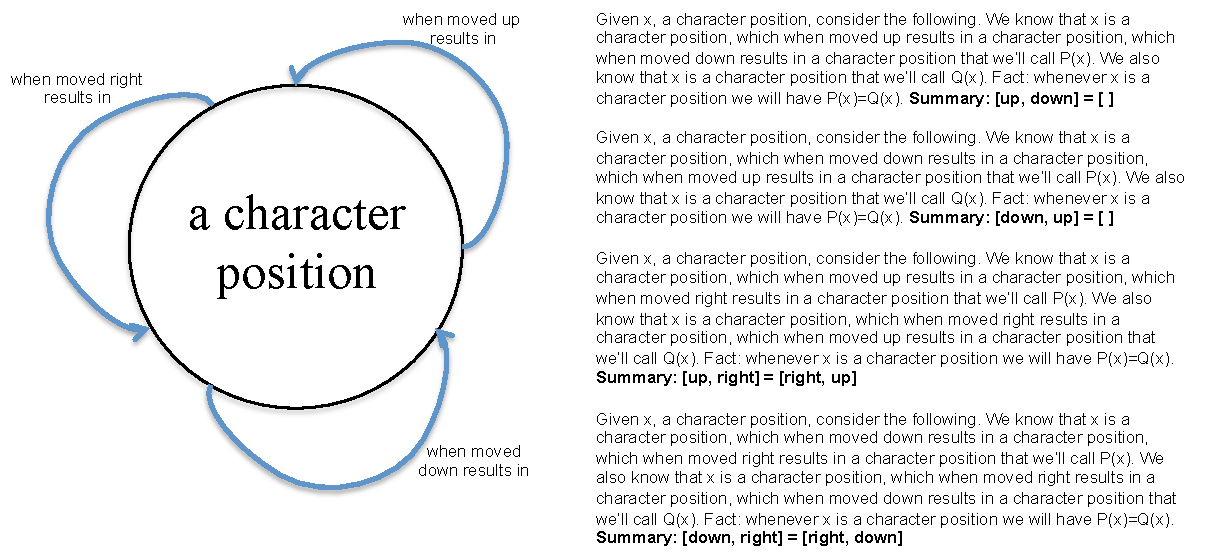
\includegraphics[width=\textwidth]{monoidOlog}
\end{center}
\end{exampleENG}

\begin{exampleRUS}\label{ex:monoid as olog}\index{моноид!олог}\index{олог!моноида}
В этом примере мы покажем, как сопоставить олог действию моноида. Рассмотрим моноид $M,$ порожденный множеством $\{u,d,r\},$ элементы которого означают «вверх, вниз, вправо», удовлетворяющий отношениям
$$[u,d]\sim[\,],\hsp[d,u]\sim[\,],\hsp[u,r]=[r,u],\hsp \tn{и}\hsp [d,r]=[r,d].$$
Мы пожем представить, как $M$ действует на множестве положений персонажа в старой видеоигре. В данном случае олог, соответствующий этому действию, должен выглядеть примерно так:
\begin{center}
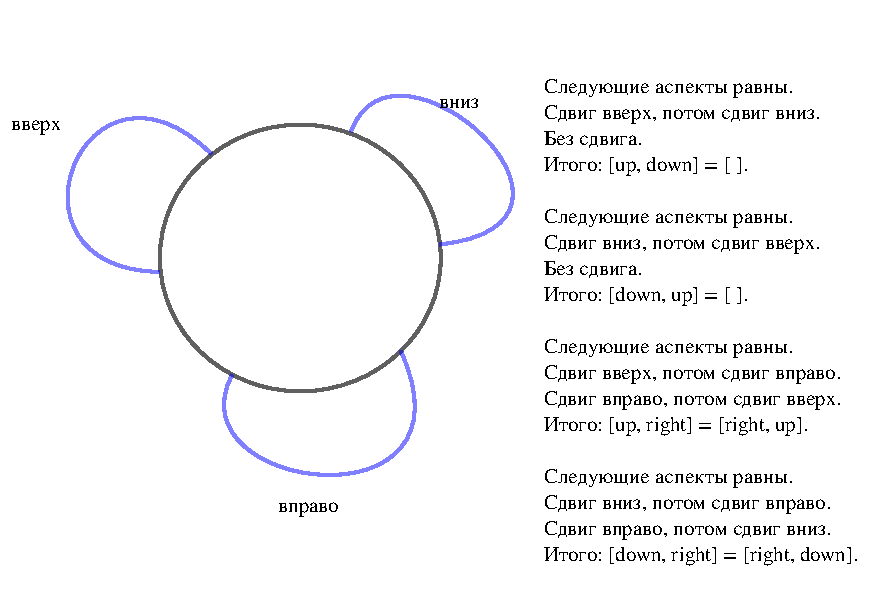
\includegraphics[width=\textwidth]{monoidOlogRU}
\end{center}
\end{exampleRUS}

%% Subsubsection %%

\subsubsection{\caseENGRUS{Finite state machines}{ / }{Конечные автоматы}}\label{sec:FSMs}

\begin{blockENG}
According to Wikipedia, a \href{http://en.wikipedia.org/wiki/Finite_state_machine#Mathematical_model}{\em deterministic finite state machine} is a quintuple $(\Sigma,S,s_0,\delta,F),$ where
\begin{enumerate}
\item $\Sigma$ is a finite non-empty set of symbols, called the {\em input alphabet},
\item $S$ is a finite, non-empty set, called {\em the state set},
\item $\delta\taking \Sigma\times S\to S$ is a function, called the {\em state-transition function}, and
\item $s_0\in S$ is an element, called {\em the initial state},
\item $F\ss S$ is a subset, called the {\em set of final states}.
\end{enumerate}
\end{blockENG}

\begin{blockRUS}
Согласно Википедии, \href{https://ru.wikipedia.org/wiki/%D0%9A%D0%BE%D0%BD%D0%B5%D1%87%D0%BD%D1%8B%D0%B9_%D0%B0%D0%B2%D1%82%D0%BE%D0%BC%D0%B0%D1%82#.D0.94.D0.B5.D1.82.D0.B5.D1.80.D0.BC.D0.B8.D0.BD.D0.B8.D1.80.D0.BE.D0.B2.D0.B0.D0.BD.D0.BD.D0.BE.D1.81.D1.82.D1.8C}{\em детерминированный конечный автомат} — это пятерка $(\Sigma,S,s_0,\delta,F),$ где
\begin{enumerate}
\item $\Sigma$ — конечное непустое множество символов, называемое {\em входным алфавитом},
\item $S$ — конечное непустое множество, называемое {\em множеством состояний},
\item $\delta\taking \Sigma\times S\to S$ — функция, называемая {\em функцией переходов},
\item $s_0\in S$ — элемент, называемый {\em начальным состоянием},
\item $F\ss S$ — подмножество, называемое {\em множеством финальных состояний}.
\end{enumerate}
\end{blockRUS}

\begin{blockENG}
In this book we will not worry about the initial state and the set of final states, concerning ourselves more with the interaction via $\delta$ of the alphabet $\Sigma$ on the set $S$ of states.
\end{blockENG}

\begin{blockRUS}
В данной книге нас не будут заботить начальное состояние и множество финальных состояний, мы больше сосредоточимся на воздействии алфавита $\Sigma$ на множество $S$ состояний при помощи $\delta$.
\end{blockRUS}

\begin{figure}[h]
\begin{center}
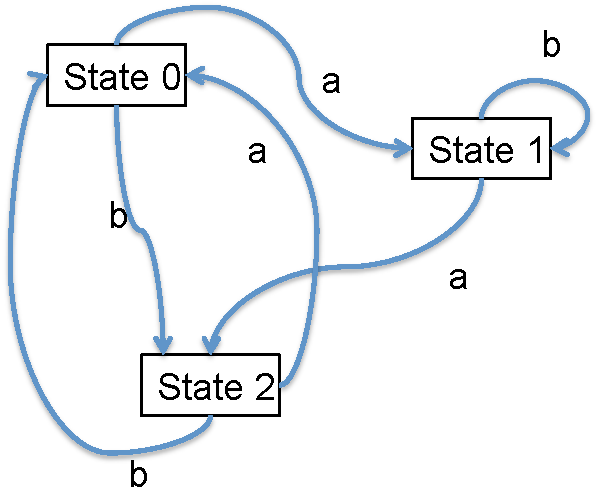
\includegraphics[height=2in]{FSM1}
\end{center}
\begin{blockENG}
\caption{A finite state machine with alphabet $\Sigma=\{a,b\}$ and state set $S=\{\tn{State 0, State 1, State 2}\}.$ If pressed, we will make State 0 the initial state and \{State 2\} the set of final states.}\label{fig:fsa}
\end{blockENG}
\begin{blockRUS}
\caption{Конечный автомат с алфавитом $\Sigma=\{a,b\}$ и множеством состояний $S=\{\tn{State 0, State 1, State 2}\}.$ В случае необходимости можно сделать состояние State 0 начальным, а \{State 2\} выбрать в качестве множества финальных состояний.}\label{fig:fsa}
\end{blockRUS}
\end{figure}

\begin{blockENG}
The following proposition expresses the notion of finite state automata in terms of free monoids and their actions on finite sets.
\end{blockENG}

\begin{blockRUS}
Следующее утверждение выражает понятие конечного автомата в терминах свободных моноидов и их действий на конечных множествах.
\end{blockRUS}

\begin{propositionENG}\index{finite state machine}
Let $\Sigma, S$ be finite non-empty sets. Giving a function $\delta\taking\Sigma\times S\to S$ is equivalent to giving an action of the free monoid $\List(\Sigma)$ on $S.$
\end{propositionENG}

\begin{propositionRUS}\index{конечный автомат}
Пусть $\Sigma, S$ — это конечные непустые множества. Задание функции $\delta\taking\Sigma\times S\to S$ эквивалентно заданию действия свободного моноида $\List(\Sigma)$ на $S.$
\end{propositionRUS}

\begin{proofENG}
By Definition~\ref{def:monoid action}, we know that function $\epsilon\taking\List(\Sigma)\times S\to S$ constitutes an action of the monoid $\List(\Sigma)$ on the set $S$ if and only if, for all $s\in S$ we have $\epsilon([\,],s)=s,$ and for any two elements $m,m'\in\List(\Sigma)$ we have $\epsilon(m,\epsilon(m',s))=\epsilon(m\star m',s),$ where $m\star m'$ is the concatenation of lists. Let $$A=\{\epsilon\taking \List(\Sigma)\times S\to S\|\epsilon\tn{ constitutes an action}\}.$$ We need to prove that there is an isomorphism of sets $$\phi\taking A\To{\iso}\Hom_\Set(\Sigma\times S,S).$$

Given an element $\epsilon\taking\List(\Sigma)\times S\to S$ in $A,$ define $\phi(\epsilon)$ on an element $(\sigma,s)\in\Sigma\times S$ by $\phi(\epsilon)(\sigma,s):=\epsilon([\sigma],s),$ where $[\sigma]$ is the one-element list. We now define $\psi\taking\Hom_\Set(\Sigma\times S,S)\to A.$

Given an element $f\in\Hom_\Set(\Sigma\times S,S),$ define $\psi(f)\taking\List(\Sigma)\times S\to S$ on a pair $(L,s)\in\List(\Sigma)\times S,$ where $L=[\epsilon_1,\ldots,\epsilon_n]$ as follows. By induction, if $n=0,$ put $\psi(f)(L,s)=s$; if $n\geq 1,$ let $L'=[\epsilon_1,\ldots,\epsilon_{n-1}]$ and put $\psi(f)(L,s)=\psi(f)(L',f(\epsilon_n,s)).$ One checks easily that $\psi(f)$ satisfies the two rules above, making it an action of $\List(\Sigma)$ on $S.$ It is also easy to check that $\phi$ and $\psi$ are mutually inverse, completing the proof.
\end{proofENG}

\begin{proofRUS}
Из Определения~\ref{def:monoid action} мы знаем, что функция $\varepsilon\taking\List(\Sigma)\times S\to S$ образует действие моноида $\List(\Sigma)$ на множестве $S$ ттт для всех $s\in S$ выполняется $\varepsilon([\,],s)=s$ и для любых двух элементов $m,m'\in\List(\Sigma)$ выполняется $\varepsilon(m,\varepsilon(m',s))=\varepsilon(m\star m',s),$ где $m\star m'$ — это конкатенация списков. Пусть $$A=\{\varepsilon\taking \List(\Sigma)\times S\to S\|\varepsilon\tn{ образует действие}\}.$$ Нам требуется доказать, что имеется изоморфизм множеств $$\varphi\taking A\To{\iso}\Hom_\Set(\Sigma\times S,S).$$

Для данного элемента $\varepsilon\taking\List(\Sigma)\times S\to S$ в $A$ зададим значение $\varphi(\varepsilon)$ на элементе $(\sigma,s)\in\Sigma\times S$ как $\varphi(\varepsilon)(\sigma,s):=\varepsilon([\sigma],s),$ где $[\sigma]$ — одноэлементный список. Теперь определим $\psi\taking\Hom_\Set(\Sigma\times S,S)\to A.$

Для данного элемента $f\in\Hom_\Set(\Sigma\times S,S)$ зададим $\psi(f)\taking\List(\Sigma)\times S\to S$ на паре $(L,s)\in\List(\Sigma)\times S,$ где $L=[\varepsilon_1,\ldots,\varepsilon_n]$ следующим образом. По индукции, если $n=0,$ положим $\psi(f)(L,s):=s$; если $n\geq 1,$ обозначим $L'=[\varepsilon_1,\ldots,\varepsilon_{n-1}]$ и зададим $\psi(f)(L,s):=\psi(f)(L',f(\varepsilon_n,s)).$ Можно легко проверить, что $\psi(f)$ удовлетворяет двум вышеупомянутым условиям, образуя действие $\List(\Sigma)$ на $S.$ Также легко проверить, что $\varphi$ и $\psi$ взаимно обратны, что завершает доказательство.
\end{proofRUS}

\begin{blockENG}
We sum up the idea of this section as follows:
\begin{sloganENG}
A finite state machine is an action of a free monoid on a finite set.
\end{sloganENG}
\end{blockENG}

\begin{blockRUS}
Мы подведем итог идее этого раздела так:
\begin{sloganRUS}
Конечный автомат — это действие свободного моноида на конечном множестве.
\end{sloganRUS}
\end{blockRUS}

\begin{exerciseENG}
Consider the functions $\phi$ and $\psi$ above.
\sexc Show that for any $f\taking\Sigma\times S\to S,$ the map $\psi(f)\taking\List(\Sigma)\times S\to S$ constitutes an action.
\item Show that $\phi$ and $\psi$ are mutually inverse functions (i.e. $\phi\circ\psi=\id_{\Hom(\Sigma\times S,S)}$ and $\psi\circ\phi=\id_{A}.$)
\endsexc
\end{exerciseENG}

\begin{exerciseRUS}
Рассмотрим функции $\varphi$ и $\psi,$ определенные выше.
\sexc Покажите, что для любых $f\taking\Sigma\times S\to S,$ отображение $\psi(f)\taking\List(\Sigma)\times S\to S$ задает действие.
\item Покажите, что $\varphi$ и $\psi$ являются взаимно обратными функциями (например, $\varphi\circ\psi=\id_{\Hom(\Sigma\times S,S)}$ и $\psi\circ\varphi=\id_{A}.$)
\endsexc
\end{exerciseRUS}

%%%% Subsection %%%%

\subsection{\caseENGRUS{Monoid action tables}{ / }{Таблицы действия моноидов}}\label{sec:monoid action table}

\begin{blockENG}
Let $M$ be a monoid generated by the set $G=\{g_1,\ldots,g_m\},$ and with some relations, and suppose that $\alpha\taking M\times S\to S$ is an action of $M$ on a set $S=\{s_1,\ldots,s_n\}.$ We can represent the action $\alpha$ using an {\em action table} whose columns are the elements of $G$ and whose rows are the elements of $S.$ In each cell $(row,col),$ where $row\in S$ and $col\in G,$ we put the element $\alpha(col,row)\in S.$
\end{blockENG}

\begin{exampleENG}[Action table]\label{ex:action table}\index{action table}
If $\Sigma$ and $S$ are the sets from Figure~\ref{fig:fsa}, the displayed action of $\List(\Sigma)$ on $S$ would be given by the action table
\begin{align}\label{dia:action table for FSM}
\begin{tabular}{| l || l | l |}\bhline
\multicolumn{3}{|c|}{Action from~\ref{fig:fsa}}\\\bhline
{\bf ID}&{\bf a}&{\bf b}\\\bbhline
State 0&State 1&State 2\\\hline
State 1& State 2& State 1\\\hline
State 2&State 0&State 0\\\bhline
\end{tabular}
\end{align}
\end{exampleENG}

\begin{exampleRUS}[Action table]\label{ex:action table}\index{таблица действия}
\end{exampleRUS}

\begin{exampleENG}[Multiplication action table]\label{ex:multiplication table}
Every monoid acts on itself by its multiplication formula, $M\times M\to M.$ If $G$ is a generating set for $M,$ we can write the elements of $G$ as the columns and the elements of $M$ as rows, and call this a multiplication table. For example, let $(\NN,1,*)$ denote the multiplicative monoid of natural numbers. The multiplication table is as follows:
\begin{align}
\begin{tabular}{| l || l | l | l | l | l | l | l |}\bhline
\multicolumn{8}{|c|}{Multiplication of natural numbers}\\\bhline
{\bf $\NN$}&{\bf 0}&{\bf 1}&{\bf 2}&{\bf 3}&{\bf 4}&{\bf 5}&{\bf $\cdots$}\\\bbhline
0&0&0&0&0&0&0&$\cdots$\\\hline
1&0&1& 2& 3 & 4&5&$\cdots$\\\hline
2&0&2&4&6&8&10&$\cdots$\\\hline
3&0&3&6&9&12&15&$\cdots$\\\bhline
4&0&4&8&12&16&20&$\cdots$\\\bhline
\vdots&\vdots&\vdots&\vdots&\vdots&\vdots&\vdots&$\ddots$\\\hline
21&0&21&42&63&84&105&$\cdots$\\\hline
\vdots&\vdots&\vdots&\vdots&\vdots&\vdots&\vdots&$\ddots$\\\bhline
\end{tabular}
\end{align}
Try to understand what is meant by this: “applying column $2$ and then column $2$ returns the same thing as applying column $4.$”

In the above table, we were implicitly taking every element of $\NN$ as a generator (since we had a column for every natural number). In fact, there is a smallest generating set for the monoid $(\NN,1,*),$ so that every element of the monoid is a product of some combination of these generators, namely the primes and 0.
\begin{align*}
\begin{tabular}{| l || l | l | l | l | l | l | l |}\bhline
\multicolumn{8}{|c|}{Multiplication of natural numbers}\\\bhline
{\bf $\NN$}&{\bf 0}&{\bf 2}&{\bf 3}&{\bf 5}&{\bf 7}&{\bf 11}&{\bf $\cdots$}\\\bbhline
0&0&0&0&0&0&0&$\cdots$\\\hline
1&0&2& 3& 5 & 7&11&$\cdots$\\\hline
2&0&4&6&10&14&22&$\cdots$\\\hline
3&0&6&9&15&21&33&$\cdots$\\\bhline
4&0&8&12&20&28&44&$\cdots$\\\bhline
\vdots&\vdots&\vdots&\vdots&\vdots&\vdots&\vdots&$\ddots$\\\hline
21&0&42&63&105&147&231&$\cdots$\\\hline
\vdots&\vdots&\vdots&\vdots&\vdots&\vdots&\vdots&$\ddots$\\\bhline
\end{tabular}
\end{align*}
\end{exampleENG}

\begin{exampleRUS}[Multiplication action table]\label{ex:multiplication table}
\end{exampleRUS}

\begin{exerciseENG}
Let $\NN$ be the additive monoid of natural numbers, let $S=\{0,1,2,\ldots,11\},$ and let $\cdot\taking\NN\times S\to S$ be the action given in Example~\ref{ex:clocks}. Using a nice small generating set for the monoid, write out the corresponding action table.
\end{exerciseENG}

\begin{exerciseRUS}
\end{exerciseRUS}

%%%% Subsection %%%%

\subsection{\caseENGRUS{Monoid homomorphisms}{ / }{Гомоморфизмы моноидов}}

\begin{blockENG}
A monoid $(M,e,\star)$ involves a set, an identity element, and a multiplication formula. For two monoids to be comparable, their sets, their identity elements, and their multiplication formulas should be appropriately comparable.\index{appropriate comparison} For example the additive monoids $\NN$ and $\ZZ$ should be comparable because $\NN\ss\ZZ$ is a subset, the identity elements in both cases are the same $e=0,$ and the multiplication formulas are both integer addition.
\end{blockENG}

\begin{definitionENG}\label{def:monoid hom}\index{monoid!homomorphism}
Let $\mcM:=(M,e,\star)$ and $\mcM':=(M',e',\star')$ be monoids. A {\em monoid homomorphism $f$ from $\mcM$ to $\mcM'$}, denoted $f\taking\mcM\to\mcM',$ is a function $f\taking M\to M'$ satisfying two conditions:
\begin{itemize}
\item $f(e)=e',$ and
\item $f(m_1\star m_2)=f(m_1)\star'f(m_2),$ for all $m_1,m_2\in M.$
\end{itemize}
The set of monoid homomorphisms from $\mcM$ to $\mcM'$ is denoted $\Hom_{\Mon}(\mcM,\mcM').$
\end{definitionENG}

\begin{definitionRUS}\label{def:monoid hom}\index{monoid!homomorphism}
\end{definitionRUS}

\begin{exampleENG}[From $\NN$ to $\ZZ$]\label{ex:nat to int}
As stated above, the inclusion map $i\taking\NN\to\ZZ$ induces a monoid homomorphism $(\NN,0,+)\to(\ZZ,0,+)$ because $i(0)=0$ and $i(n_1+n_2)=i(n_1)+i(n_2).$

Let $i_5\taking\NN\to\ZZ$ denote the function $i_5(n)=5*n,$ so $i_5(4)=20.$ This is also a monoid homomorphism because $i_5(0)=5*0=0$ and $i_5(n_1+n_2)=5*(n_1+n_2)=5*n_1+5*n_2=i_5(n_1)+i_5(n_2).$
\end{exampleENG}

\begin{exampleRUS}[From $\NN$ to $\ZZ$]\label{ex:nat to int}
\end{exampleRUS}

\begin{applicationENG}\label{app:RNA reader 1}
Let $R=\{a,c,g,u\}$ and let $T=R^3,$ the set of triplets in $R.$ Let $\mcR=\List(R)$ be the free monoid on $R$ and let $\mcT=\List(T)$ denote the free monoid on $T.$ There is a monoid homomorphism $F\taking\mcT\to\mcR$ given by sending $t=(r_1,r_2,r_3)$ to the list $[r_1,r_2,r_3].$
\footnote{More precisely, the monoid homomorphism $F$ sends a list $[t_1,t_2,\ldots,t_n]$ to the list $[r_{1,1},r_{1,2},r_{1,3},r_{2,1},r_{2,2},r_{2,3},\ldots,r_{n,1},r_{n,2},r_{n,3}],$ where for each $0\leq i\leq n$ we have $t_i=(r_{i,1},r_{i,2},r_{i,3}).$}

If $A$ be the set of amino acids and $\mcA=\List(A)$ the free monoid on $A,$ the process of \href{http://en.wikipedia.org/wiki/Translation_(biology)}{\text translation} gives a monoid homomorphism $G\taking\mcT\to\mcA,$ turning a list of RNA triplets into a polypeptide. But how do we go from a list of RNA nucleotides to a polypeptide? The answer is that there is no good way to do this mathematically. So what is going wrong?

The answer is that there should not be a monoid homomorphism $\mcR\to\mcA$ because not all sequences of nucleotides produce a polypeptide; for example if the sequence has only two elements, it does not code for a polypeptide. There are several possible remedies to this problem. One is to take the image of $F,$ which is a submonoid $\mcR'\ss\mcR.$ It is not hard to see that there is a monoid homomorphism $F'\taking\mcR'\to\mcT,$ and we can compose it with $G$ to get our desired monoid homomorphism $G\circ F'\taking\mcR'\to\mcA.$
\footnote{Adding stop-codons to the mix we can handle more of $\mcR,$ e.g. sequences that don't have a multiple-of-three many nucleotides.}
\end{applicationENG}

\begin{applicationRUS}\label{app:RNA reader 1}
\end{applicationRUS}

\begin{exampleENG}\label{ex:trivial monoid homomorphism}\index{monoid!trivial homomorphism}
Given any monoids $\mcM$ there is a unique monoid homomorphism from $\mcM$ to the trivial monoid $\ul{1}$ (see Example~\ref{ex:trivial monoid}). There is also a unique homomorphism $\ul{1}\to\mcM.$ These facts together have an upshot: between any two monoids $\mcM$ and $\mcM'$ we can always construct a homomorphism
$$\mcM\Too{!}\ul{1}\Too{!}\mcM'$$
which we call the {\em trivial homomorphism $\mcM\to\mcM'$}.\index{trivial homomorphism!of monoids} A morphism $\mcM\to\mcM'$ that is not trivial is called a {\em nontrivial homomorphism}.
\end{exampleENG}

\begin{exampleRUS}\label{ex:trivial monoid homomorphism}\index{monoid!trivial homomorphism}
\end{exampleRUS}

\begin{propositionENG}\label{prop:int to nat trivial}
Let $\mcM=(\ZZ,0,+)$ and $\mcM'=(\NN,0,+).$ The only monoid homomorphism $f\taking\mcM\to\mcM'$ sends every element $m\in\ZZ$ to $0\in\NN.$
\end{propositionENG}

\begin{propositionRUS}\label{prop:int to nat trivial}
\end{propositionRUS}

\begin{proofENG}
Let $f\taking\mcM\to\mcM'$ be a monoid homomorphism, and let $n=f(1)$ and $n'=f(-1)$ in $\NN.$ Then we know that since $0=1+(-1)$ in $\ZZ$ we must have $0=f(0)=f(1+(-1))=f(1)+f(-1)=n+n'\in\NN.$ But if $n\geq 1$ then this is impossible, so $n=0.$ Similarly $n'=0.$ Any element $m\in\ZZ$ can be written $m=1+1+\cdots+1$ or as $m=-1+-1+\cdots+-1,$ and it is easy to see that $f(1)+f(1)+\cdots+f(1)=0=f(-1)+f(-1)+\cdots+f(-1).$ Therefore, $f(m)=0$ for all $m\in\ZZ.$
\end{proofENG}

\begin{proofRUS}
\end{proofRUS}

\begin{exerciseENG}
For any $m\in\NN$ let $i_m\taking\NN\to\ZZ$ be the function $i_m(n)=m*n.$ All such functions are monoid homomorphisms $(\NN,0,+)\to(\ZZ,0,+).$ Do any monoid homomorphisms $(\NN,0,+)\to(\ZZ,0,+)$ not come in this way? For example, what about using $n\mapsto 5*n-1$ or $n\mapsto n^2,$ or some other function?
\end{exerciseENG}

\begin{exerciseRUS}
\end{exerciseRUS}

\begin{exerciseENG}
Let $\mcM:=(\NN,0,+)$ be the additive monoid of natural numbers, let $\mcN=(\RR_{\geq0},0,+)$ be the additive monoid of nonnegative real numbers, and let $\mcP:=(\RR_{>0},1,*)$ be the multiplicitive monoid of positive real numbers. Can you think of any nontrivial monoid homomorphisms of the following sorts: $$\mcM\to\mcN,\hsp\mcM\to\mcP,\hsp\mcN\to\mcP,\hsp \mcN\to\mcM,\hsp\mcP\to\mcN?$$
\end{exerciseENG}

\begin{exerciseRUS}
\end{exerciseRUS}


%% Subsubsection %%

\subsubsection{\caseENGRUS{Homomorphisms from free monoids}{ / }{Гомоморфизмы из свободного моноида}}

\begin{blockENG}
Recall that $(\NN,0,+)$ is the free monoid on one generator. It turns out that for any other monoid $\mcM=(M,e,\star),$ the set of monoid homomorphisms $\NN\to\mcM$ is in bijection with the set $M.$ This is a special case (in which $G$ is a set with one element) of the following proposition.
\end{blockENG}

\begin{blockRUS}
\end{blockRUS}

\begin{propositionENG}\label{prop:free monoid}
Let $G$ be a set, let $F(G):=(\List(G),[\,],\plpl)$ be the free monoid on $G,$ and let $\mcM:=(M,e,\star)$ be any monoid. There is a natural bijection
$$\Hom_\Mon(F(G),\mcM)\To{\iso}\Hom_\Set(G,M).$$
\end{propositionENG}

\begin{propositionRUS}\label{prop:free monoid}
\end{propositionRUS}

\begin{proofENG}
We provide a function $\phi\taking\Hom_\Mon(F(G),\mcM)\to\Hom_\Set(G,M)$ and a function $\psi\taking\Hom_\Set(G,M)\to\Hom_\Mon(F(G),\mcM)$ and show that they are mutually inverse. Let us first construct $\phi.$ Given a monoid homomorphism $f\taking F(G)\to\mcM,$ we need to provide $\phi(f)\taking G\to M.$ Given any $g\in G$ we define $\phi(f)(g):=f([g]).$

Now let us construct $\psi.$ Given $p\taking G\to M,$ we need to provide $\psi(p)\taking\List(G)\to\mcM$ such that $\psi(p)$ is a monoid homomorphism. For a list $L=[g_1,\ldots,g_n]\in\List(G),$ define $\psi(p)(L):=p(g_1)\star\cdots\star p(g_n)\in M.$ In particular, $\psi(p)([\,])=e.$ It is not hard to see that this is a monoid homomorphism. It is also easy to see that $\phi\circ\psi(p)=p$ for all $p\in\Hom_\Set(G,M).$ We show that $\psi\circ\phi(f)=f$ for all $f\in\Hom_\Mon(F(G),\mcM).$ Choose $L=[g_1,\ldots,g_n]\in\List(G).$ Then
$$\psi(\phi f)(L)=(\phi f)(g_1)\star\cdots\star(\phi f)(g_n)=f[g_1]\star\cdots\star f[g_n]=f([g_1,\ldots,g_n])=f(L).$$
\end{proofENG}

\begin{proofRUS}
\end{proofRUS}

\begin{exerciseENG}
Let $G=\{a,b\},$ let $\mcM:=(M,e,\star)$ be any monoid, and let $f\taking G\to M$ be given by $f(a)=m$ and $f(b)=n,$ where $m,n\in M.$ If $\psi\taking\Hom_\Set(G,M)\to\Hom_\Mon(F(G),\mcM)$ is the function from the proof of Proposition~\ref{prop:free monoid} and $L=[a,a,b,a,b],$ what is $\psi(f)(L)$ ?
\end{exerciseENG}

\begin{exerciseRUS}
\end{exerciseRUS}

%% Subsubsection %%

\subsubsection{\caseENGRUS{Restriction of scalars}{ / }{Ограничение скаляров}}

\begin{blockENG}
A monoid homomorphism $f\taking M\to M'$ (see Definition~\ref{def:monoid hom}) ensures that the elements of $M$ have a reasonable interpretation in $M'$; they act the same way over in $M'$ as they did back home in $M.$ If we have such a homomorphism $f$ and we have an action $\alpha\taking M'\times S\to S$ of $M'$ on a set $S,$ then we have a method for allowing $M$ to act on $S$ as well. Namely, we take an element of $M,$ send it over to $M',$ and act on $S.$ In terms of functions, we compose $\alpha$ with the function $f\times\id_S\taking M\times S\to M'\times S,$ to get a function we'll denote $$\Delta_f(\alpha)\taking M\times S\to S.$$ After Proposition~\ref{prop:restriction of scalars} we will know that $\Delta_f(\alpha)$ is indeed a monoid action, and we say that it is given by {\em restriction of scalars along $f$}.\index{restriction of scalars}
\end{blockENG}

\begin{blockRUS}
\end{blockRUS}

\begin{propositionENG}\label{prop:restriction of scalars}
Let $\mcM:=(M,e,\star)$ and $\mcM':=(M',e',\star')$ be monoids, $f\taking\mcM\to\mcM'$ a monoid homomorphism, $S$ a set, and suppose that $\alpha\taking M'\times S\to S$ is an action of $\mcM'$ on $S.$ Then $\Delta_f(\alpha)\taking M\times S\to S,$ defined as above, is a monoid action as well.
\end{propositionENG}

\begin{propositionRUS}\label{prop:restriction of scalars}
\end{propositionRUS}

\begin{proofENG}
Refer to Remark~\ref{rmk:monoid action}; we assume $\alpha$ is a monoid action and want to show that $\Delta_f(\alpha)$ is too. We have $\Delta_f(\alpha)(e,s)=\alpha(f(e),s)=\alpha(e',s)=s.$ We also have
\begin{align*}
\Delta_f(\alpha)(m,\Delta_f(\alpha)(n,s))=\alpha(f(m),\alpha(f(n),s))&=\alpha(f(m)\star' f(n),s)\\
&=\alpha(f(m\star n),s)\\
&=\Delta_f(\alpha)(m\star n,s).
\end{align*}
\end{proofENG}

\begin{proofRUS}
\end{proofRUS}

\begin{exampleENG}
Let $\NN$ and $\ZZ$ denote the additive monoids of natural numbers and integers, respectively, and let $i\taking\NN\to\ZZ$ be the inclusion, which we saw in Example~\ref{ex:nat to int} is a monoid homomorphism. There is an action $\alpha\taking\ZZ\times\RR\to\RR$ of the monoid $\ZZ$ on the set $\RR$ of real numbers, given by $\alpha(n,x)=n+x.$ Clearly, this action works just as well if we restrict our scalars to $\NN\ss\ZZ,$ allowing ourselves only to add natural numbers to reals. The action $\Delta_i\alpha\taking\NN\times\RR\to\RR$ is given on $(n,x)\in\NN\times\RR$ by $\Delta_i\alpha(n,x)=\alpha(i(n),x)=\alpha(n,x)=n+x,$ just as expected.
\end{exampleENG}

\begin{exampleRUS}
\end{exampleRUS}

\begin{exampleENG}
Suppose that $V$ is a complex vector space. In particular, this means that the monoid $\CC$ of complex numbers (under multiplication) acts on the elements of $V.$ If $i\taking\RR\to\CC$ is the inclusion of the real line inside $\CC,$ then $i$ is a monoid homomorphism. Restriction of scalars in the above sense turns $V$ into a real vector space, so the name “restriction of scalars” is apt.
\end{exampleENG}

\begin{exampleRUS}
\end{exampleRUS}

\begin{exerciseENG}
Let $\NN$ be the free monoid on one generator, let $\Sigma=\{a,b\},$ and let $S=\{\tn{State 0, State 1, State 2}\}.$ Consider the map of monoids $f\taking\NN\to\List(\Sigma)$ given by sending $1\mapsto [a,b,b].$ The monoid action $\alpha\taking\List(\Sigma)\times S\to S$ given in Example~\ref{ex:action table} can be transformed by restriction of scalars along $f$ to an action $\Delta_f(\alpha)$ of $\NN$ on $S.$ Write down its action table.
\end{exerciseENG}

\begin{exerciseRUS}
\end{exerciseRUS}

\end{document}
